% =====================================================================
% CHAPTER 1 -- Summary of: A. Freni et al., Electronics, 2023 [Freni2023]
% =====================================================================
\section*{CHAPTER 1. CURVED SES ON URBAN LIGHT POLES}
\addcontentsline{toc}{section}{\numberline{}CHAPTER 1. CURVED SES ON URBAN LIGHT POLES}
\setcounter{section}{1}
\setcounter{subsection}{0}
\setcounter{equation}{0}
\setcounter{theorem}{0}
\setcounter{figure}{0}
\setcounter{table}{0}

\subsection{Problem}
Fifth-generation (5G) links in the millimeter-wave (mmWave) band suffer from high free-space and building-penetration losses and are easily blocked by obstacles. Areas without line of sight (LOS) to the base station (BS) may therefore receive almost no signal~\cite{Freni2023}. Adding BSs fixes this but raises cost, network complexity, visual impact and electromagnetic pollution. Smart electromagnetic skins (SESs) are a cheaper alternative: thin passive surfaces that re-radiate the incident field towards a non-specular direction. However, SESs are usually conceived as planar panels on building walls, which is often impossible. The wall may face the wrong way relative to the BS, be covered with windows, or belong to a protected historic building~\cite{Freni2023}.

\subsection{Contributions and Methodology}
Freni \textit{et al.}~\cite{Freni2023} propose installing a \emph{curved} SES on existing street-light or traffic-light poles, hidden inside a cylindrical radome. According to the authors, this is the first performance analysis of such a solution in a real urban scenario. Fig.~\ref{fig:ch1-geometry} shows the geometry. The SES sits between a pole of 240~mm diameter and a radome of at most 300~mm diameter, with a minimum curvature radius of 175~mm and a horizontal aperture of $96^\circ$. Its equivalent planar size is $300 \times 340$~mm (about $27.5\lambda_0 \times 31\lambda_0$ at 27.5~GHz), discretized into $55 \times 62$ unit cells.

\begin{figure}[!htbp]
    \centering
    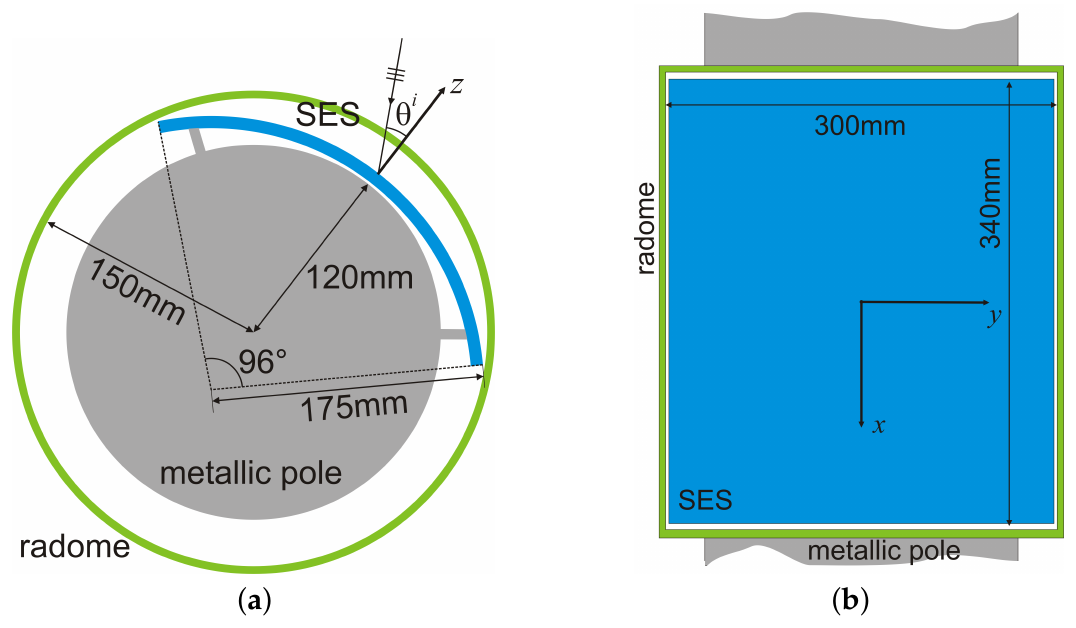
\includegraphics[width=0.8\textwidth]{Images/ch1_freni_fig3.png}
    \caption[Geometry of the curved SES on a light pole]{Geometry of the curved SES placed between the metallic pole and the cylindrical radome: (a) top view, (b) lateral view (adapted from~\cite{Freni2023}).}
    \label{fig:ch1-geometry}
\end{figure}

Each cell is a square metallic patch of side $W$ on a 0.8~mm grounded DiClad527 substrate ($\varepsilon_r = 2.55$, $\tan\delta = 0.0022$), with a 5.45~mm period ($\lambda_0/2$ at 27.5~GHz); the substrate is thin enough to be bent. The curvature radius is large (about $15\lambda$ at 26~GHz), so the cell response is computed with an infinite periodic model, which the authors cross-checked against finite planar and curved $5 \times 5$ arrays. The phase delay that the $ij$-th cell must introduce is~\cite{Freni2023}
\begin{equation}\label{eq:ch1-phase}
\Delta\varphi_{ij} = k_0\,\hat{\mathbf{k}}'\cdot\mathbf{r}'_{ij} - k_0\,\hat{\mathbf{k}}\cdot\mathbf{r}'_{ij} + f(u_i,v_j) + \varphi_0 ,
\end{equation}
where $k_0$ is the free-space wavenumber, $\hat{\mathbf{k}}'$ the direction of the incident plane wave, $\mathbf{r}'_{ij}$ the center of the $ij$-th element, $f(u_i,v_j)$ the desired phase distribution on a plane $uv$ orthogonal to the unit vector $\hat{\mathbf{k}}$, and $\varphi_0$ an arbitrary constant (Fig.~\ref{fig:ch1-problem}). With a uniform $f$, \eqref{eq:ch1-phase} produces a pencil beam along $\hat{\mathbf{k}}$. For street coverage, $f$ is instead synthesized with Powell's direction-set algorithm to obtain a cosecant-squared beam. All results are full-wave simulations (CST Microwave Studio) in the Italian 5G band, 26.5--27.5~GHz.

\begin{figure}[!htbp]
    \centering
    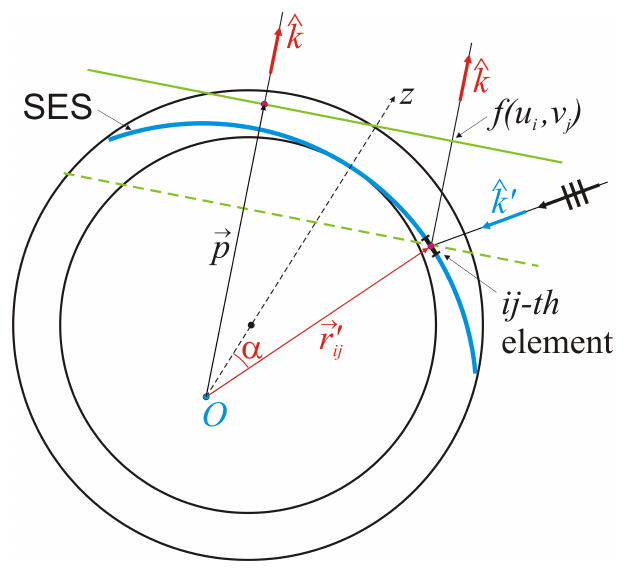
\includegraphics[width=0.55\textwidth]{Images/ch1_freni_fig6.png}
    \caption[Geometry of the phase-delay calculation]{Geometry of the phase-delay calculation in \protect\eqref{eq:ch1-phase}: incident direction $\hat{\mathbf{k}}'$, desired direction $\hat{\mathbf{k}}$, center $\mathbf{r}'_{ij}$ of the $ij$-th element, and phase distribution $f(u_i,v_j)$ on the plane orthogonal to $\hat{\mathbf{k}}$ (adapted from~\cite{Freni2023}).}
    \label{fig:ch1-problem}
\end{figure}

\subsection{Limitations of the Approach}
\begin{itemize}
    \item The square-patch cell covers only about $290^\circ$ of reflection phase instead of $360^\circ$, because $W$ must stay between 1 and 4~mm to avoid a resonance near 4.6~mm. The required phase is therefore only approximated on part of the surface, which degrades performance~\cite{Freni2023}.
    \item On a curved surface the local incidence angle varies from cell to cell. Even at normal incidence on the central cell, the maximum incidence angle on the elements is $47^\circ$, and it increases by $\theta^i$ when the wave arrives obliquely~\cite{Freni2023}.
    \item The BS field is modelled as a plane wave (far-field illumination), and the study is purely numerical: no prototype was built or measured.
\end{itemize}

\subsection{Results and Evaluation}
Table~\ref{tab:ch1-results} compares the curved SES with two planar SESs of the same height mounted on the same pole. The curved SES never gives a lower maximum radar cross section (RCS) than the planar SES that fits in the same cylindrical radome, and it is about 3~dB higher at 27~GHz~\cite{Freni2023}. The reason is the usable aperture: the curved skin uses the whole arc between pole and radome, while a flat skin tangent to the pole is limited to 180~mm. A flat skin as wide as the chord (262~mm) gains less than 1~dB more. However, it can only be installed by cutting the pole or using a custom-shaped radome, which adds cost and visual impact. Over 26.5--27.5~GHz the maximum RCS of the curved SES varies by less than 1~dB.

At 27~GHz, a quarter-wave radome lowers the RCS by 0.9~dB for polytetrafluoroethylene (PTFE, $\tan\delta = 0.0002$) and by 1.2~dB for Lexan ($\tan\delta = 0.01$). The larger drop with Lexan follows from its 50 times higher loss tangent. A $\pm 3^\circ$ error in the incidence angle tilts the beam (a larger incidence angle gives a smaller pointing angle), but the pattern keeps its shape within $\pm 2^\circ$. Installers can therefore fine-tune the coverage by rotating or shifting the SES on the pole.

In the urban case study, the SES stands 45~m from the BS, with incidence $\theta^i = 20^\circ$, and shapes a cosecant-squared beam towards a street at $30^\circ$ that is not in LOS of the BS. The power densities are computed as~\cite{Freni2023}
\begin{equation}\label{eq:ch1-power}
S_i = \frac{\mathrm{EIRP}}{4\pi \Delta_{\mathrm{BS\text{-}SES}}^2}, \qquad S_s = \frac{S_i\,\mathrm{RCS}(\hat{\mathbf{R}})}{4\pi R^2},
\end{equation}
where $S_i$ is the power density incident on the SES, $\Delta_{\mathrm{BS\text{-}SES}}$ the BS--SES distance, $\mathrm{EIRP} = 1$~W the effective isotropic radiated power (EIRP) of the BS, $S_s$ the power density scattered to a ground point, and $R$ and $\hat{\mathbf{R}}$ the distance and direction of that point from the SES. The first expression is printed in~\cite{Freni2023} without the square on $\Delta_{\mathrm{BS\text{-}SES}}$; the square is restored here, because a power density must fall with the square of the distance, as the second expression does. According to \eqref{eq:ch1-power}, the scattered power density is about 20~dB lower than the density radiated directly by the BS, because the small SES intercepts only a small part of the BS power. It is nevertheless the only signal reaching the street, and it is enough for a stable link. Ripples in the shaped beam come from diffraction at the SES edges, since the plane wave illuminates the whole surface uniformly.

\begin{table}[!htbp]
    \centering
    \caption[Curved versus planar SESs in the same pole--radome volume]{Curved SES versus planar SESs of the same height mounted on the same pole at 27~GHz; RCS values are relative to the curved SES~\cite{Freni2023}.}
    \label{tab:ch1-results}
    \small
    \begin{tabularx}{\textwidth}{l >{\raggedright\arraybackslash}X >{\raggedright\arraybackslash}X >{\raggedright\arraybackslash}X}
        \toprule
        Configuration & Horizontal size (cells) & Radome & Maximum RCS \\
        \midrule
        Curved SES (proposed) & 300~mm arc, 262~mm chord (55) & cylindrical, 300~mm diameter & reference \\
        Planar, tangent to pole & 180~mm (33) & cylindrical, 300~mm diameter & about $-3$~dB \\
        Planar, chord width & 262~mm (48) & custom shaped & less than $+1$~dB \\
        \bottomrule
    \end{tabularx}
\end{table}

\subsection{Open Issues and Future Directions}
The authors leave the optimization of the unit cell towards a full $360^\circ$ phase range to future work~\cite{Freni2023}. Two more gaps follow from the results. First, the design still needs experimental validation with a fabricated curved prototype and a real BS. Second, size trades off against visual impact: a larger skin would raise the scattered power, now about 20~dB below the direct field, but also its visibility. Finally, the beam is fixed and can only be adjusted by a few degrees during installation; Chapter~2 removes this limitation with a rotatable design.
